\section{Develop and draw logic circuit with 4 inputs that will only produce logic 1 when only exactly 2 inputs are logic 1.}
    \subsection{Sử dụng phương pháp bìa Karnaugh.}
        \hspace*{-2.2cm}Sử dụng phương pháp bìa Karnaugh, ta có bảng sau:\\[0.2cm]
            \begin{centering}
                \begin{tabular}{|c|c|c|c|c|}
                    \hline
                    \diagbox{CD}{AB} & 00 & 01 & 11 & 10 \\
                    \hline
                    00 & 0 & 0 & 1 & 0 \\
                    \hline
                    01 & 0 & 1 & 0 & 1 \\
                    \hline
                    11 & 1 & 0&  0 & 0 \\
                    \hline
                    10 & 0 & 1 & 0 & 1 \\
                    \hline
                \end{tabular}\\[0.5cm]
            \end{centering}
            $\Rightarrow$ Hàm logic: $F = \overline{A}.\overline{B}.C.D + A.B.\overline{C}.\overline{D} + \overline{A}.B.\overline{C}.D + A.\overline{B}.C.\overline{D} + \overline{A}.B.C.\overline{D} + A.\overline{B}.\overline{C}.D$ 
    \subsection{Vẽ mạch bằng phần mềm Proteus.}
        \begin{figure}[H]
            \centering
            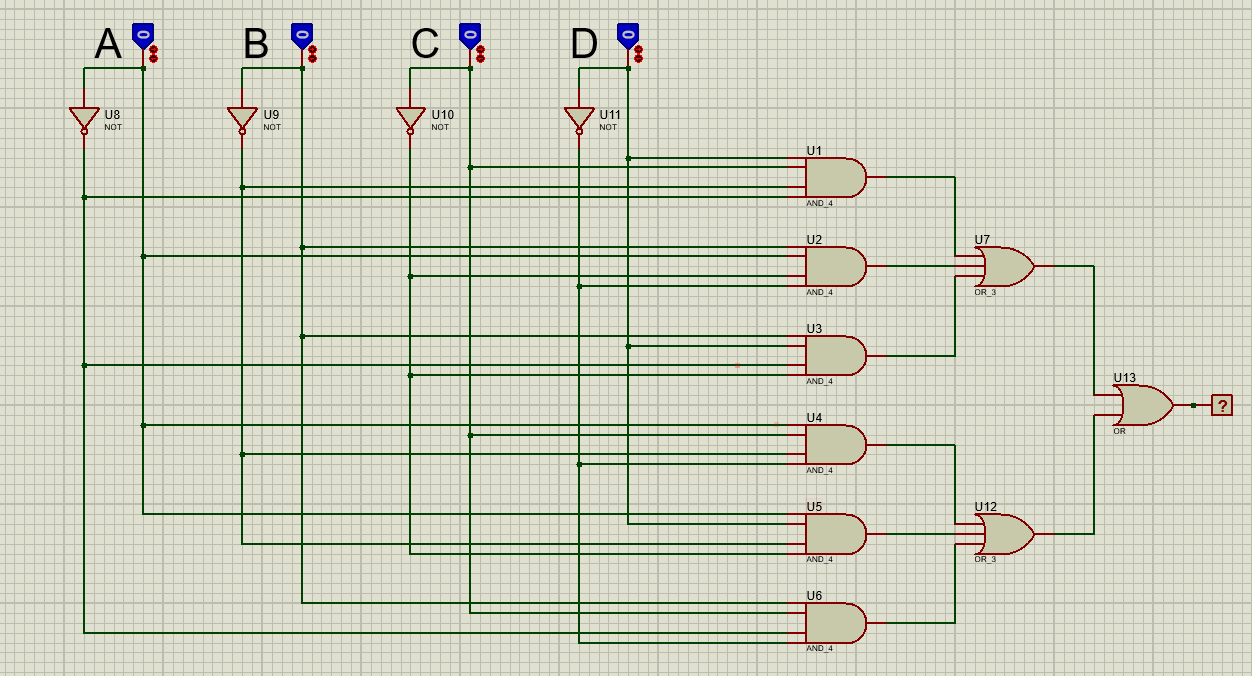
\includegraphics[width=0.8\textwidth]{pictures/b2.png}
            \caption{Mạch logic bài 2}
        \end{figure}
    \subsection{Kiểm tra lại từng trường hợp bằng mô phỏng trên phần mềm Proteus.}
        \subsubsection{Trường hợp $\overline{A}.\overline{B}.C.D$}
            \begin{figure}[H]
                \centering
                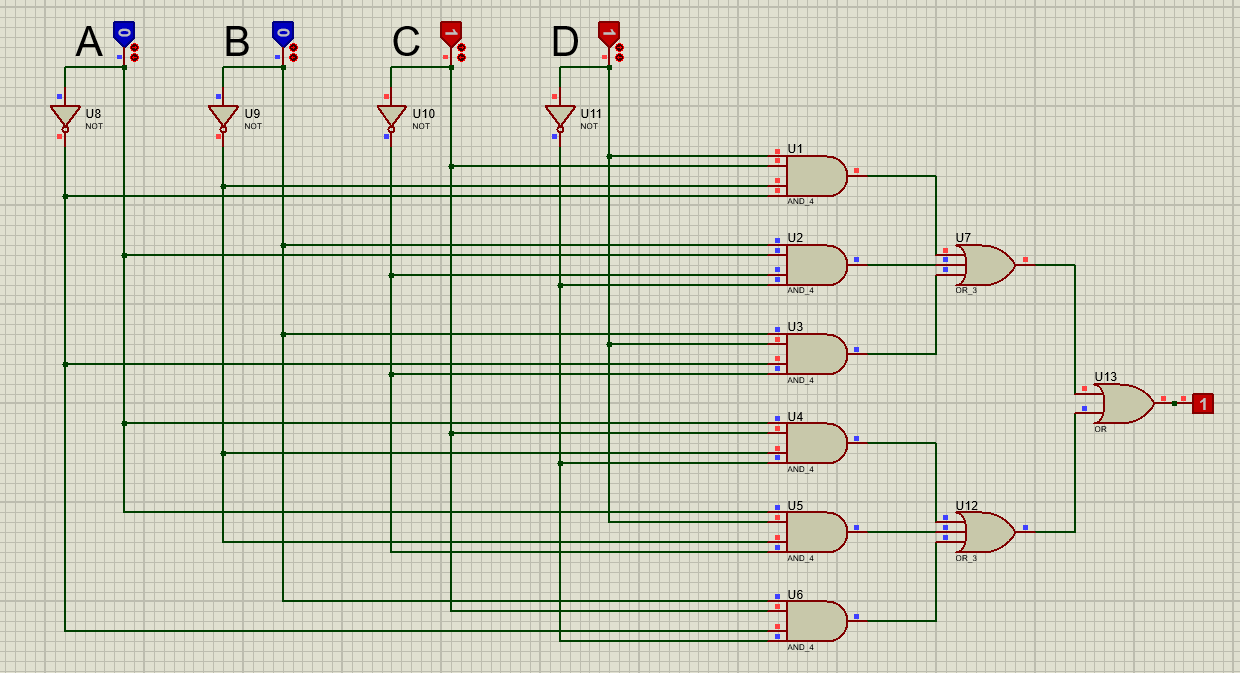
\includegraphics[width=0.8\textwidth]{pictures/b2.2.png}
                \caption{Trường hợp $\overline{A}.\overline{B}.C.D$}
            \end{figure}
        \subsubsection{Trường hợp $A.B.\overline{C}.\overline{D}$}
            \begin{figure}[H]
                \centering
                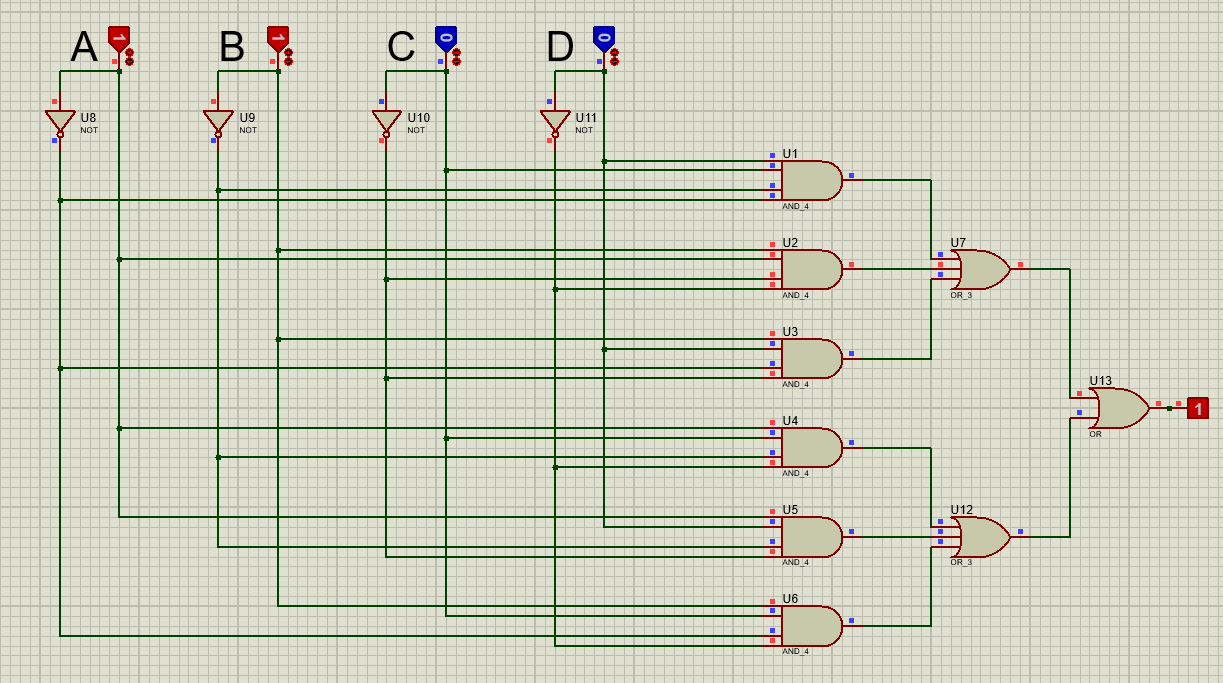
\includegraphics[width=0.8\textwidth]{pictures/b2.1.png}
                \caption{Trường hợp $A.B.\overline{C}.\overline{D}$}
            \end{figure}
        \subsubsection{Trường hợp $\overline{A}.B.\overline{C}.D$}
            \begin{figure}[H]
                \centering
                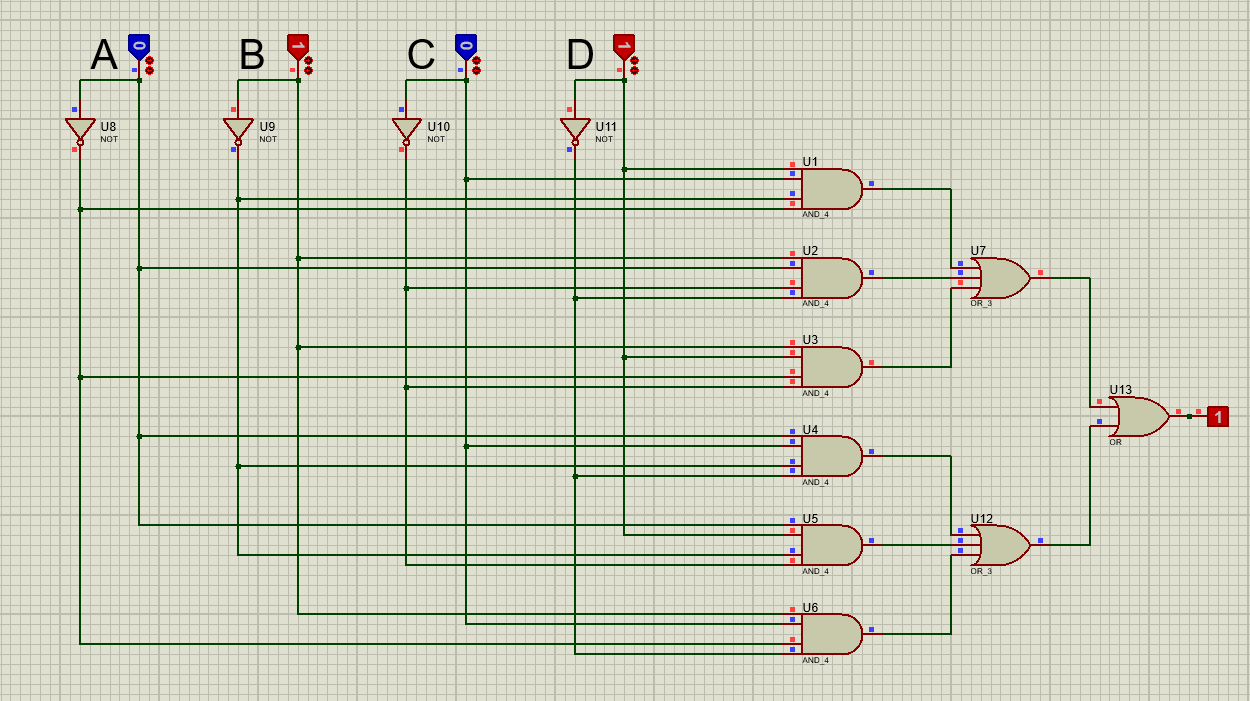
\includegraphics[width=0.8\textwidth]{pictures/b2.4.png}
                \caption{Trường hợp $\overline{A}.B.\overline{C}.D$}
            \end{figure}
        \subsubsection{Trường hợp $A.\overline{B}.C.\overline{D}$}
            \begin{figure}[H]
                \centering
                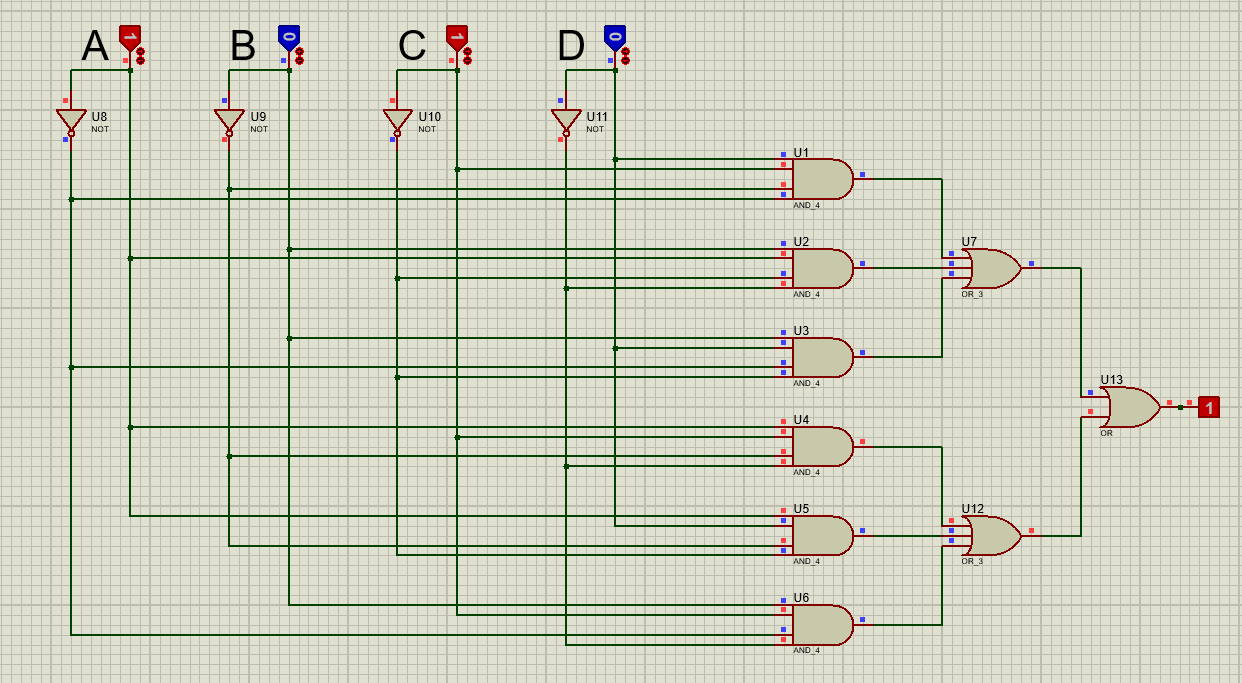
\includegraphics[width=0.8\textwidth]{pictures/b2.3.png}
                \caption{Trường hợp $A.\overline{B}.C.\overline{D}$}
            \end{figure}
        \subsubsection{Trường hợp $\overline{A}.B.C.\overline{D}$}
            \begin{figure}[H]
                \centering
                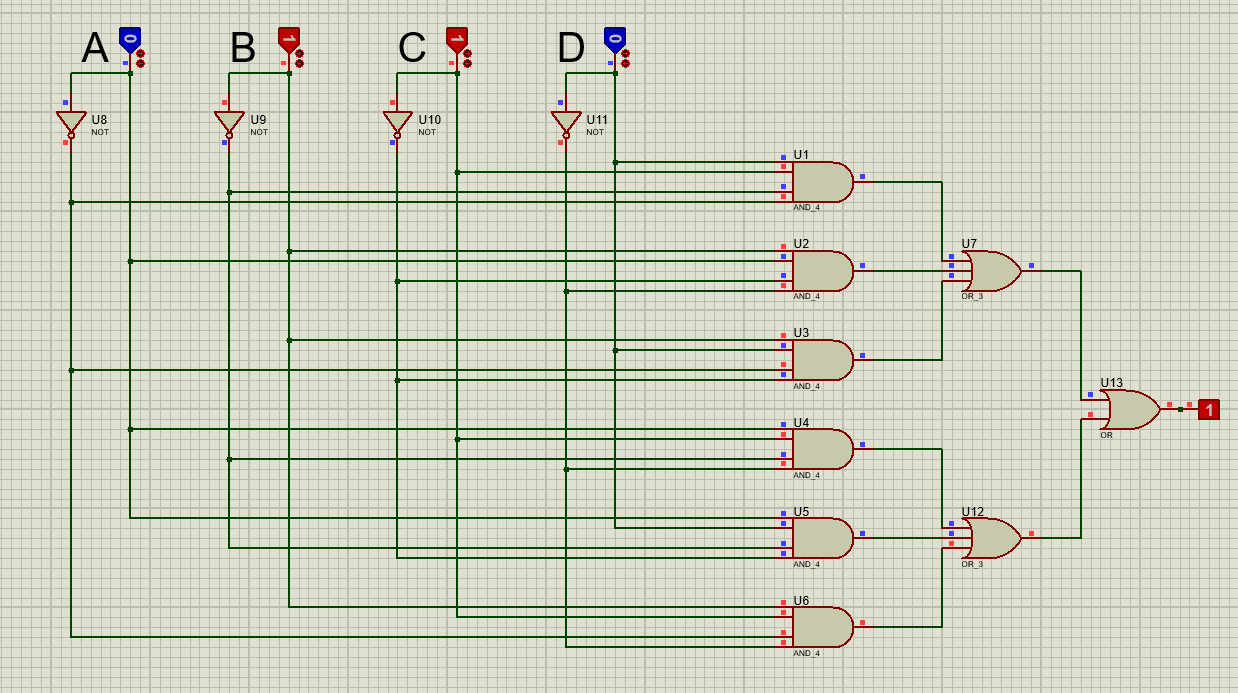
\includegraphics[width=0.8\textwidth]{pictures/b2.6.png}
                \caption{Trường hợp $\overline{A}.B.C.\overline{D}$}
            \end{figure}
        \subsubsection{Trường hợp $A.\overline{B}.\overline{C}.D$}
            \begin{figure}[H]
                \centering
                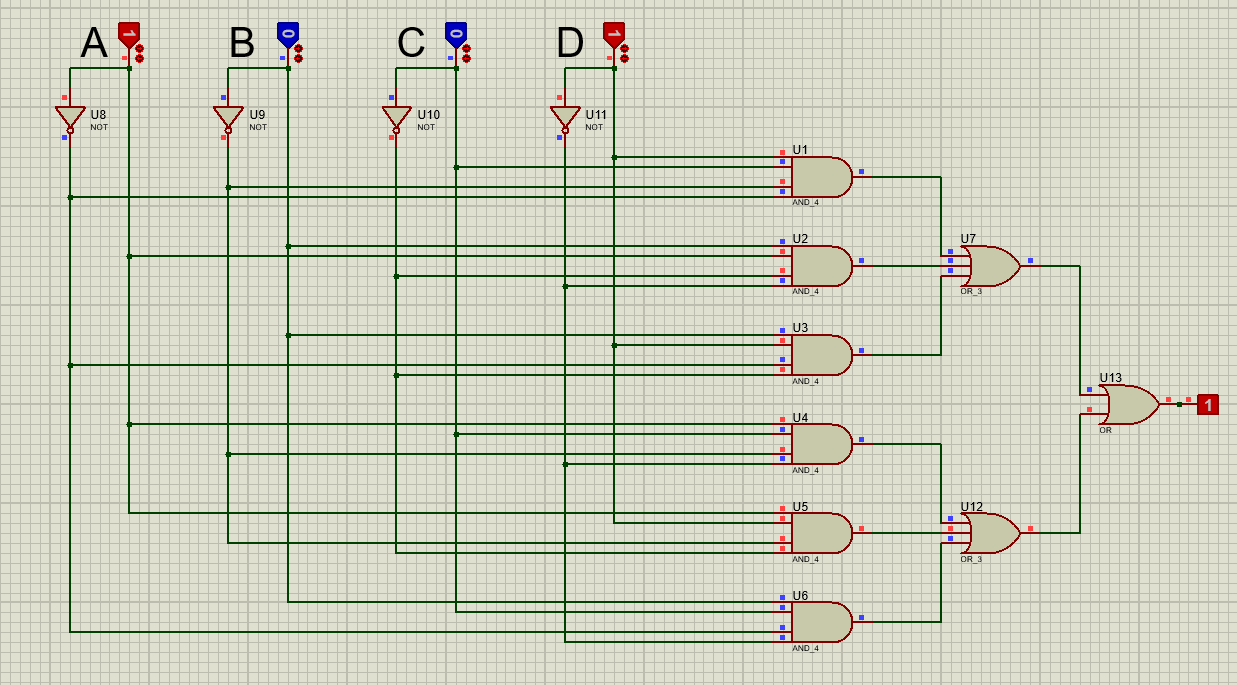
\includegraphics[width=0.8\textwidth]{pictures/b2.5.png}
                \caption{Trường hợp $A.\overline{B}.\overline{C}.D$}
            \end{figure}
